\section{Building HLG}
\label{sec:building}

\subsection{System architecture}
\label{sec:arch}

\begin{figure}[t]
    \centering
    \begin{tikzpicture}[
        node distance=1.1cm and 1.4cm,
        box/.style={draw, rounded corners=2pt, align=center, minimum width=2.6cm,
                    minimum height=0.85cm, font=\small},
        arrow/.style={-{Stealth[length=2mm]}, thick},
    ]
        \node[box] (agent) {LLM agent\\(turn / one-shot)};
        \node[box, right=of agent] (driver) {Eval driver\\\texttt{main.py}};
        \node[box, right=of driver] (validator) {Engine validator\\\texttt{OK}/\texttt{LOSS}/\texttt{WIN}};
        \node[box, below=of validator] (solver) {Dead-state BFS\\\texttt{engine/solver.py}};
        \node[box, below=of driver] (logger) {JSONL logger\\\texttt{agent\_logger.py}};

        \draw[arrow] (agent) -- node[above, font=\scriptsize]{move} (driver);
        \draw[arrow] (driver) -- node[above, font=\scriptsize]{apply} (validator);
        \draw[arrow] (validator) -- node[right, font=\scriptsize]{next state} (driver);
        \draw[arrow] (driver) -- node[left, font=\scriptsize]{events} (logger);
        \draw[arrow, dashed] (solver) -- node[above, font=\scriptsize]{post-move lookup} (driver);
    \end{tikzpicture}
    \caption{HLG system architecture. The main loop consults the agent each turn,
    receives a proposed move, and forwards it to the game engine's validator, which
    returns the next state and an \texttt{OK}/\texttt{LOSS}/\texttt{WIN} status. Logged
    events flow through observability into JSONL traces. Dead-state detection runs as
    an offline BFS pass per level (bottom-right) and is consulted post-move; it does
    \emph{not} live inline in the validator.}
    \label{fig:arch}
\end{figure}

\subsection{Production pipeline}

HLG is small enough that a heavyweight studio model is not warranted. The pipeline is
linear:

\begin{enumerate}[leftmargin=1.5em]
    \item \textbf{Source levels.} 34 \texttt{.txt} grids drawn from
      grahambarrgraham's repository \cite{grahambarrgrahambloxorz}.
    \item \textbf{Parse.} \texttt{engine/state.py} tokenizes each level into a tile
      grid and a switch / teleport wiring table.
    \item \textbf{Verify.} \texttt{verify\_solutions.py} replays a known-optimal
      action sequence per level and asserts the engine reports \texttt{WIN}.
    \item \textbf{Precompute dead states.} \texttt{engine/solver.py} runs forward BFS
      from the initial state, records reverse edges, then runs backward BFS from
      WIN-adjacent states. Reachable states not in the backward closure are dead.
    \item \textbf{LLM harness.} The agent drivers in \texttt{main.py} run the engine
      against a model API, in either turn or one-shot mode, optionally chained via
      sequence mode.
\end{enumerate}

\subsection{Engine}

The engine is dependency-free Python. Three modules:
\begin{itemize}[leftmargin=1.5em]
    \item \texttt{engine/state.py} parses level files and computes the next block
      position given a direction (a pure function of the current orientation).
    \item \texttt{engine/validator.py} applies a move and returns
      \texttt{(status, next\_state)}. It checks boundary, missing-tile, and
      weak-tile-upright conditions; it activates strong, weak, and teleport tiles; and it
      handles split mode (two-target teleports) including the merge logic for
      reuniting the halves.
    \item \texttt{engine/solver.py} computes the per-level dead-state set via
      two-phase BFS.
\end{itemize}

We accurately disclose the following: the validator currently does \emph{not} consult
the dead-state set in-line. A \texttt{TODO} marker at line 42 of
\texttt{engine/validator.py} flags this as future work. The driver in \texttt{main.py}
performs the lookup explicitly after each move and tags the attempt with
\texttt{[DEAD]} rather than \texttt{[LOSS]}. This separation keeps the validator
provably side-effect-free with respect to history-dependent solver caches.

\subsection{Environment design constraints}

\begin{itemize}[leftmargin=1.5em]
    \item \textbf{Mechanic diversity}: the 34 levels collectively exercise plain
      tiles, weak tiles, both switch types, single- and two-target teleports, and split
      mode.
    \item \textbf{Move-count diversity}: optimal solution lengths range from 7 to
      113. Difficulty as measured by optimal length is approximately monotone in
      level index.
    \item \textbf{Verifiable correctness}: every level has a reference solution
      replayed in \texttt{verify\_solutions.py}; corrupting a level breaks CI.
\end{itemize}

\subsection{Automated validation}

The validation pipeline has three layers:
\begin{enumerate}[leftmargin=1.5em]
    \item \emph{Solution replay.} Each level's reference solution is replayed; a
      \texttt{WIN} is required.
    \item \emph{Dead-state computation.} Each level's dead-state set is computed at
      driver startup. The BFS terminates within seconds per level.
    \item \emph{Random-policy probe.} A uniformly random policy is run for $N$ steps
      against every level; non-tutorial levels must not be solvable by chance.
\end{enumerate}

\subsection{Dataset composition}
\label{sec:dataset}

\begin{table}[h]
\centering
\caption{HLG dataset composition. Tutorial level 0 is excluded from official scoring.
Optimal lengths $L_l$ are taken from \texttt{verify\_solutions.py}.}
\label{tab:dataset}
\begin{tabular}{@{}lrrrr@{}}
\toprule
\textbf{Subset} & \textbf{Levels} & \textbf{$N$} & \textbf{$L_l$ range} & \textbf{Notes} \\
\midrule
Tutorial      & 0          & 1  & --            & No mechanics; single open arena. \\
Public Demo   & 1--9       & 9  & 7--34         & No switches before level 8. \\
Semi-Private  & 10--24     & 15 & 33--82        & Used for the official leaderboard. \\
Fully-Private & 25--33     & 9  & 51--128       & Reserved for the HLG Challenge. \\
\midrule
Total         &            & 34 & 7--128        & \\
\bottomrule
\end{tabular}
\end{table}


\begin{figure}[h]
    \centering
    \begin{subfigure}{0.45\linewidth}
        \centering
        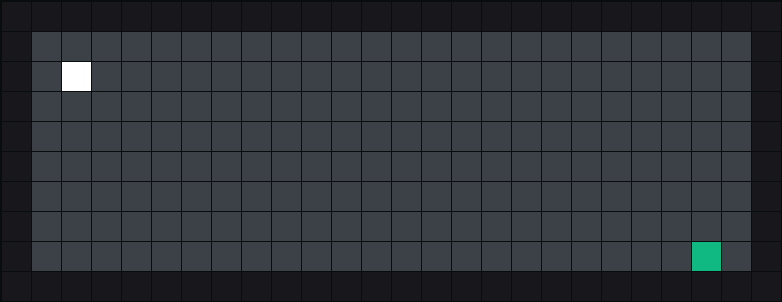
\includegraphics[width=\linewidth]{figures/level0.png}
        \caption{Level 0 — tutorial. No mechanics; the agent only navigates from start (purple) to end (green).}
    \end{subfigure}
    \hfill
    \begin{subfigure}{0.45\linewidth}
        \centering
        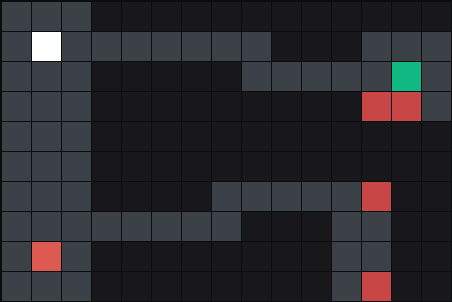
\includegraphics[width=\linewidth]{figures/level17.png}
        \caption{Level 17 — multiple bridge groups and weak tiles. Optimal solution has 104 moves.}
    \end{subfigure}
    \caption{Two levels at the extremes of the difficulty curve. The block (white) starts on the purple start tile and must end UPRIGHT on the green end tile. Red tiles are switches; muted-red tiles are weak.}
    \label{fig:levels}
\end{figure}
